\chapter{Statistiek}
\begin{exercises}{}{
    \begin{enumerate}[noitemsep, label=\textbf{\arabic*}.]
    \item Bereken die gemiddelde, die mediaan en die modus van die volgende datastelle:
      \begin{enumerate}[noitemsep, label=\textbf{(\alph*)} ]
      \item $2;~5;~8;~8;~11;~13;~22;~23;~27$
      \item $15;~17;~24;~24;~26;~28;~31;~43$
      \item $4;~11;~3;~15;~11;~13;~25;~17;~2;~11$
      \item $24;~35;~28;~41;~32;~49;~31$
      \end{enumerate}
    \item Die ouderdomme van $15$ drawwers van die  Comrades Marathon is aangeteken:
      \begin{equation*}
        31;~42;~28;~38;~45;~51;~33;~29;~42;~26;~34;~56;~33;~46;~41
      \end{equation*}
      Bereken die gemiddelde, die mediaan en die modus van die ouderdomme.
    \item In die eerste van ’n aantal flesse is daar $1$ lekkertjie. In die tweede is daar $3$ lekkers. Die gemiddelde van die aantal lekkers in die eerste twee flesse is $2$.
      \begin{enumerate}[noitemsep, label=\textbf{(\alph*)} ]
      \item As die gemiddelde aantal lekkers in die eerste drie flesse $3$ is, hoeveel lekkers is daar in die derde fles?
      \item As die gemiddelde aantal lekkers in die eerste vier flesse $4$ is, hoeveel lekkers is daar in die vierde fles?
      \end{enumerate}
    \item Vind ’n stel van 5 ouderdomme waarvoor die gemiddelde ouderdom $5$ is, die modale ouderdom (dus die modus) $2$ is en die mediaan ouderdom $3$ jaar is.
    \item Vier vriende het elkeen ’n aantal albasters. Hulle bereken dat $10$ die gemiddelde is van die aantal albasters wat hulle het. Een van hulle vertrek. Sy het $4$ albasters. Hoeveel albasters het die oorblywende vriende altesaam?
    \end{enumerate}
}
\end{exercises}


 \begin{solutions}{}{
\begin{enumerate}[itemsep=5pt, label=\textbf{\arabic*}. ] 


\item %solution1
      \begin{enumerate}[noitemsep, label=\textbf{(\alph*)} ]
\item Gemiddelde $= 13,2$; ~Mediaan $= 11$; ~Modus $= 8$ %$2;~5;~8;~8;~11;~13;~22;~23;~27$
\item Gemiddelde $= 26$; ~Mediaan $= 25$; ~Modus $= 24$%$15;~17;~24;~24;~26;~28;~31;~43$
\item Gemiddelde $=11,2$; ~Mediaan $= 11$; ~Modus $=11$%$4;~11;~3;~15;~11;~13;~25;~17;~2;~11$
\item Gemiddelde $=34,29$; ~Mediaan $=32$; ~Geen modus%$24;~35;~28;~41;~32;~49;~31$
    \end{enumerate}
\item %solution2
Gemiddelde $=38,3$; Mediaan $= 38$; Modus $= 33$ en $42$\\
\item %solution3
       \begin{enumerate}[noitemsep, label=\textbf{(\alph*)} ]
\item Laat $n_3$ die nommer lekkers in die derde fles wees:\\
$\frac{1+3+n_3}{3}=3\\
1+3+n_3=9\\
n_3=5$\\

\item Laat $n_4$ die nommer lekkers in die vierdie fles wees:\\
$\frac{1+3+5+n_4}4=4\\
9+n_4=16\\
n_4=7$
    \end{enumerate}

\item %solution 4
Laat die vyf verskillende oudedomme $x_1,~x_2,~x_3,~x_4$ en $x_5$ wees.\\
Dus is die gemiddelde\\

$\frac{x_1+x_2+x_3+x_4+x_5}{5}=5\\
x_1+x_2+x_3+x_4+x_5=25\\$
 
Die mediaan waarde is by posisie $3$, dus $x_3=3$.\\

Die modus is die oudedom wat die meeste voorkom. Daar is ten minste $2$ ourderdomme wat $2$ is. Die ander ouderdomme moet alles verskillend wees. Die vier onbekende ourderdomme kan nie almal $2$ wees, want dit sal nie 'n gemiddelde van $5$ gee. Verder, aangesien al die berekeninge van die gemiddelde, modus and mediaan is op geordende stelle data gedoen, kan ons nie $3$ ouderdomme wat $2$ is, want dan sou die mediaan ourderdom nie $2$ wees nie. Dus het ons \\

$2+2+3+x_4+x_5=25\\
18=x_4+x_5$\\

$x_4$ en $x_5$ kan enige getalle wees wat tot $18$ voeg en nie dieselfde waarde is nie, byvoorbeeld $12$ en $6$ of $8$ en $10$ of $3$ en $15$, ens.\\

Moontlik datastelle:\\
$2, 2, 3, 3, 15; ~~
2, 2, 3, 4, 14; ~~ 
2, 2, 3, 5, 13; ~~ 
2, 2, 3, 6, 12; ~~
2, 2, 3, 7, 11; ~~ 
2, 2, 3, 8, 10$\\

Let op dat die stel ouderdomme moet geordende wees, die mediaan waarde moet $3$ wees en daar moet $2$ ouderdomme van $2$ wees.\\



\item %solution 5
Laat die getal albasters per vriend $x_1,~x_2,~x_3 $ en $ x_4$ wees.\\
$\frac{x_1+x_2+x_3+x_4}{4}=10\\
x_1+x_2+x_3+x_4=40$\\
Een vriend verlaat, \\
$x_1+x_2+x_3=40−4\\
x_1+x_2+x_3=36$\\

Dus het die oorblywende vriende $36$ albasters.

\end{enumerate}}
\end{solutions}

\begin{exercises}{}{
    \begin{enumerate}[itemsep=5pt, label=\textbf{\arabic*}. ]
    \item ’n Eksperiment is onderneem in die skool en $50$ leerders is gevra om te raai hoeveel lekkers daar in ’n bottel is. Die volgende raaiskote word aangeteken:
      \\
      \begin{center}
        \begin{tabular}{|c|c|c|c|c|c|c|c|c|c|} \hline
          56 & 49 & 40 & 11 & 33 & 33 & 37 & 29 & 30 & 59 \\ \hline
          21 & 16 & 38 & 44 & 38 & 52 & 22 & 24 & 30 & 34 \\\hline
          42 & 15 & 48 & 33 & 51 & 44 & 33 & 17 & 19 & 44 \\\hline
          47 & 23 & 27 & 47 & 13 & 25 & 53 & 57 & 28 & 23 \\\hline
          36 & 35 & 40 & 23 & 45 & 39 & 32 & 58 & 22 & 40 \\\hline
        \end{tabular}
      \end{center}
      \vspace{8pt}\\

      \begin{enumerate}[noitemsep, label=\textbf{(\alph*)} ]
      \item Trek ’n gegroepeerde frekwensietabel op en gebruik die volgende intervalle
        $10 < x \leq 20$;\ $20 < x \leq 30$;\ $30 < x \leq 40$;\ 
        $40 < x \leq 50$; en \ $50 < x \leq 60$.
      \item Trek ’n histogram om die frekwensietabel van die gegroepeerde data voor te stel.
      \end{enumerate}
    \end{enumerate}
}
\end{exercises}


 \begin{solutions}{}{
\begin{enumerate}[itemsep=6pt, label=\textbf{\arabic*}. ] 
\item
%  Draw up a grouped frequency table using the intervals
%   $10 < x \leq 20$;\ $20 < x \leq 30$;\ $30 < x \leq 40$;\ 
%   $40 < x \leq 50$;and \ $50 < x \leq 60$.
\begin{enumerate}[itemsep=6pt, label=\textbf{(\alph*)} ]
% \begin{center}
\item 
\scalebox{1}{
  \begin{tabular}{|c|c|}\hline
\textbf{Groep} & \textbf{Frek} \\ \hline
$11 - 20$ &$6$\\\hline
$21 - 30$&$13$\\\hline
$31 - 40$&$15$\\\hline
$41 - 50$&$9$\\\hline
$51 - 60$&$7$\\\hline
   
  \end{tabular}}

% \end{center}

\item %Draw the histogram corresponding to the frequency table of the   grouped data.
\scalebox{0.8} % Change this value to rescale the drawing.
{
\begin{pspicture}(0,-5.0875)(8.385716,5.0475)
\definecolor{color5165b}{rgb}{0.7725490196078432,0.7725490196078432,0.7725490196078432}
\rput(1.385716,-3.9525){\psaxes[linewidth=0.028222222,arrowsize=0.05291667cm 2.0,arrowlength=1.4,arrowinset=0.4,tickstyle=bottom,ticksize=0.10583333cm,dx=1.0cm,dy=1.0cm,Dx=10,Dy=2]{<->}(0,0)(-1,-1)(7,8)}
\psframe[linewidth=0.02,dimen=outer,fillstyle=solid,fillcolor=color5165b](3.3998826,0.0475)(2.3798826,-3.9490623)
\psframe[linewidth=0.02,dimen=outer,fillstyle=solid,fillcolor=color5165b](4.419883,2.6675)(3.3798826,-3.9490623)
\psframe[linewidth=0.02,dimen=outer,fillstyle=solid,fillcolor=color5165b](5.419883,3.6075)(4.379883,-3.9490623)
\psframe[linewidth=0.02,dimen=outer,fillstyle=solid,fillcolor=color5165b](6.399883,0.6875)(5.379883,-3.9490623)
\psframe[linewidth=0.02,dimen=outer,fillstyle=solid,fillcolor=color5165b](7.399883,-0.4125)(6.379883,-3.9490623)
% \usefont{T1}{ptm}{m}{n}
\rput(4.9245706,-4.8625){\LARGE Reeks van raaiskote}
% \usefont{T1}{ptm}{m}{n}
\rput{89.854546}(0.62033606,0.27754468){\rput(0.13573046,0.46597877){\LARGE Telling}}
\end{pspicture} 
}
\end{enumerate}
\end{enumerate}}
\end{solutions}


\begin{exercises}{}{
  \begin{enumerate}[itemsep=8pt, label=\textbf{\arabic*}.]

  \item Oorweeg die volgende gegroepeerde data en bereken die gemiddelde, die modale groep en die mediaangroep.
\\
    \begin{center}
      \begin{tabular}{|c|c|}\hline
      
        \textbf{Massa (kg)} & \textbf{Telling} \\\hline
     
        $40 < m \leq 45$ & $7$ \\\hline
        $45 < m \leq 50$ & $10$ \\\hline
        $50 < m \leq 55$ & $15$ \\\hline
        $55 < m \leq 60$ & $12$ \\\hline
        $60 < m \leq 65$ & $6$ \\\hline
  
      \end{tabular}
    \end{center}

  \item Vind die gemiddelde, die modale groep en die mediaangroep in die datastel van die tyd wat mense benodig om ’n spel te voltooi:
\\
    \begin{center}
      \begin{tabular}{|c|c|} \hline

       \textbf{Tyd (s)} & \textbf{Telling} \\ \hline

        $35 < t \leq 45$ & $5$ \\\hline
        $45 < t \leq 55$ & $11$ \\\hline
        $55 < t \leq 65$ & $15$ \\\hline
        $65 < t \leq 75$ & $26$ \\\hline
        $75 < t \leq 85$ & $19$ \\\hline
        $85 < t \leq 95$ & $13$ \\\hline
        $95 < t \leq 105$ & $6$ \\\hline

      \end{tabular}
    \end{center}
% Still in English
\item Die histogram hieronder bewys die aantal passasiers wat per week in Alfred se taxi reis.\\
Bereken
\begin{enumerate}[noitemsep, label=\textbf{(\alph*)} ]
\item die modale interval
\item die totale aantal passasiers wat in Alfred se taxi gereis het
\item 'n beraming van die gemiddelde
\item 'n beraming van die mediaan
\item indien dit geskat word dat elke passasier 'n gemiddelde afstand van $5$ km gereis het, hoeveel geld sou Alfred verdien as hy R~$3,50$ per km gevra het?
\end{enumerate}
\begin{center}
\scalebox{1} % Change this value to rescale the drawing.
{
\begin{pspicture}(0,-5.1475)(9.378126,5.1075)
\definecolor{color5165b}{rgb}{0.7725490196078432,0.7725490196078432,0.7725490196078432}
\rput(1.3781264,-3.8925){\psaxes[linewidth=0.028222222,arrowsize=0.05291667cm 2.0,arrowlength=1.4,arrowinset=0.4,tickstyle=bottom,ticksize=0.10583333cm,dx=1.0cm,dy=1.0cm,Dx=100,Dy=2,Ox=300]{<->}(0,0)(-1,-1)(8,9)}
\psframe[linewidth=0.02,dimen=outer,fillstyle=solid,fillcolor=color5165b](3.392293,-1.8890625)(2.372293,-3.8890624)
\psframe[linewidth=0.02,dimen=outer,fillstyle=solid,fillcolor=color5165b](4.412293,-0.8890625)(3.372293,-3.8890624)
\psframe[linewidth=0.02,dimen=outer,fillstyle=solid,fillcolor=color5165b](5.412293,2.1309376)(4.372293,-3.8890624)
\psframe[linewidth=0.02,dimen=outer,fillstyle=solid,fillcolor=color5165b](6.392293,4.1309376)(5.372293,-3.8890624)
\psframe[linewidth=0.02,dimen=outer,fillstyle=solid,fillcolor=color5165b](7.392293,0.1309375)(6.372293,-3.8890624)
\psframe[linewidth=0.02,dimen=outer,fillstyle=solid,fillcolor=color5165b](8.392293,-2.8690624)(7.372293,-3.8890624)
% \usefont{T1}{ptm}{m}{n}
\rput(5.369637,-4.9225){Aantal passasiers}
% \usefont{T1}{ptm}{m}{n}
\rput{89.854546}(0.73185694,0.38878262){\rput(0.13573053,0.5775){Telling}}
\end{pspicture} 
}
\end{center}
  \end{enumerate}
}
\end{exercises}


 \begin{solutions}{}{
\begin{enumerate}[itemsep=5pt, label=\textbf{\arabic*}. ] 


\item Gemiddelde=$53$; Modale groep: $50<m \leq 55$; Mediaangroep: $50 < m \leq 55$
\item Gemiddelde=$71,66$; Modale groep: $65 < t \leq 75$; Mediaangroep: $65 < t \leq 75$
\item
\begin{enumerate}[noitemsep, label=\textbf{(\alph*)} ]
\item $700 < x\leq800$%the modal interval
\item $33~600$%the total number of passengers to travel in Alfred's taxi
\item $700$ %an estimate of the mean
\item $750$%an estimate of the median
\item R $588~ 000$%if it is estimated that every passenger travelled an average distance of $5$ km, how much money would Alfred have made if he charged R~$3,50$ per km?
\end{enumerate}
\end{enumerate}}
\end{solutions}

\begin{exercises}{}{
  \begin{enumerate}[noitemsep, label=\textbf{\arabic*}.]

  \item Vind die variasiewydte van die datastel:
    \begin{equation*}
      \{1;\ 2;\ 3;\ 4;\ 4;\ 4;\ 5;\ 6;\ 7;\ 8;\ 8;\ 9;\ 10;\ 10\}
    \end{equation*}

  \item Wat is die kwartiele van hierdie datastel?
    \begin{equation*}
      \{3;\ 5;\ 1;\ 8;\ 9;\ 12;\ 25;\ 28;\ 24;\ 30;\ 41;\ 50\}
    \end{equation*}

  \item ’n Klas van $12$ studente skryf ’n toets en die resultaat is as volg:
    \begin{equation*}
      20;\ 39;\ 40;\ 43;\ 43;\ 46;\ 53;\ 58;\ 63;\ 70;\ 75;\ 91
    \end{equation*}
    Vind die variasiewydte, kwartiele en die interkwartielwydte.

  \item Drie stelle data word gegee:
    \begin{itemize}  
    \item \textbf{Datastel 1:} $\{9;\ 12;\ 12;\ 14;\ 16;\ 22;\ 24\}$
    \item \textbf{Datastel 2:} $\{7;\ 7;\ 8;\ 11;\ 13;\ 15;\ 16;\ 16\}$
    \item \textbf{Datastel 3:} $\{11;\ 15;\ 16;\ 17;\ 19;\ 19;\ 22;\ 24;\ 27\}$
    \end{itemize}
    Vir elke datastel vind:
    \begin{enumerate}[noitemsep, label=\textbf{(\alph*)} ]
    \item die variasiewydte
    \item die onderste kwartiel
    \item die interkwartielwydte
    \item die semi-interkwartielwydte
    \item die mediaan
    \item die boonste kwartiel
    \end{enumerate}
  \end{enumerate}
}
\end{exercises}


 \begin{solutions}{}{
\begin{enumerate}[itemsep=5pt, label=\textbf{\arabic*}. ] 
\item Variasiewydte: $10-1=9$
\item $Q_1 = 6,2$;~ $ Q_2 = 18$;~ $Q_3 = 29$
\item Variasiewydte: $91-20=71$\\
 $Q_1 = 41,5$;~ $Q_2 = 49,5$;~ $Q_3 = 66,5$ \\
 Interkwartielwydte: $66,5-41,5=25$
\item 
\begin{enumerate}[noitemsep, label=\textbf{(\alph*)} ]
    \item Variasiewydte: $24-9=15$; $~~16-7=9$; $~~27-11=16$
    \item $Q_1$: $12$;  $7,5$; $15,5$ 
    \item Interkwartielwydte: $10$; $8$; $7,5$
    \item Semi-interkwartielwydte: $5$; $4$; $3,75$
    \item Mediaan: $14$; $12$; $19$
    \item $Q_3$: $22$; $15,5$; $23$
\end{enumerate}

\end{enumerate}}
\end{solutions}

\begin{exercises}{}{
    \begin{enumerate} [itemsep=6pt, label=\textbf{\arabic*}.]

    \item Lisa werk in ’n rekenaarwinkel. Sy verkoop die volgende aantal rekenaars in ’n maand:
      \begin{equation*}
        \{27;\ 39;\ 3;\ 15;\ 43;\ 27;\ 19;\ 54;\ 65;\ 23;\ 45;\ 16\}
      \end{equation*}
     Gee die vyf-getal opsomming en die mond-en-snor grafiek van Lisa se verkope.

    \item Zithulele werk in telefoonverkope. Hy hou boek van die aantal verkope wat hy elke maand doen en die data word hier gegee:.
      \begin{equation*}
        \{49;\ 12;\ 22;\ 35;\ 2;\ 45;\ 60;\ 48;\ 19;\ 1;\ 43;\ 12\}
      \end{equation*}
    Gee die vyf-getal opsomming en die mond-en-snor grafiek van Zithulele se verkope.

    \item Hannah het vir nege maande gewerk as ’n bloemiste. Sy verkoop die volgende aantal bruidsruikers:
      \begin{equation*}
        \{16;\ 14;\ 8;\ 12;\ 6;\ 5;\ 3;\ 5;\ 7\}
      \end{equation*}
      Gee die vyf-getal opsomming van Hannah se verkope.
    \item Gebruik die diagram hieronder om die vyf-getal opsomming te bereken:
      \begin{enumerate}[noitemsep, label=\textbf{(\alph*)} ]
      \item \raisebox{-2cm}{
          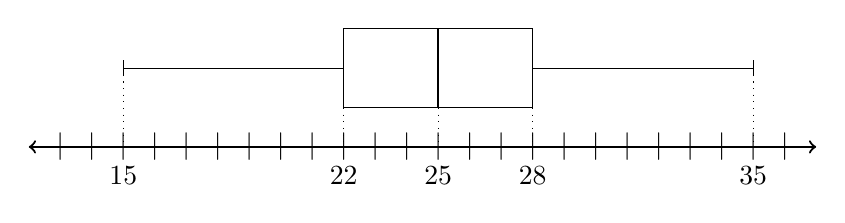
\begin{tikzpicture}[xscale=0.4]
            \def\median{25}
            \def\firstquartile{22}
            \def\thirdquartile{28}
            \def\minimum{15}
            \def\maximum{35}

            \draw (\firstquartile, -0.5 ) rectangle ( \thirdquartile,0.5);
            \draw[thick] ( \median,-0.5) -- ( \median,0.5);
            \draw (    \firstquartile, 0) -- (\minimum,0   );
            \draw ( \minimum, -0.1) -- (       \minimum, 0.1);
            \draw (  \thirdquartile, 0) -- (   \maximum, 0);
            \draw ( \maximum, -0.1) -- (      \maximum, 0.1 );

            \draw[thick,<->] (12,-1) -- (37,-1);

            \foreach \x in {\minimum, \firstquartile, \median, \thirdquartile, \maximum} {
              \draw (\x,-1.6) -- (\x, -1.6) node[anchor=south] {$\x$};
            }

            \foreach \x in {13,14,...,36} {
              \draw (\x,-1.3) -- (\x, -1.3) node[anchor=south] {$|$};
            }
            \draw[dotted] ( \maximum, 0) -- ( \maximum, -1);
            \draw[dotted] ( \thirdquartile, 0) -- ( \thirdquartile, -1);
            \draw[dotted] (\median, 0)  -- ( \median, -1);
            \draw[dotted] (\firstquartile, 0) -- ( \firstquartile, -1);
            \draw[dotted] ( \minimum, 0) -- ( \minimum, -1);
          \end{tikzpicture}
        }
      \item \raisebox{-2cm}{
          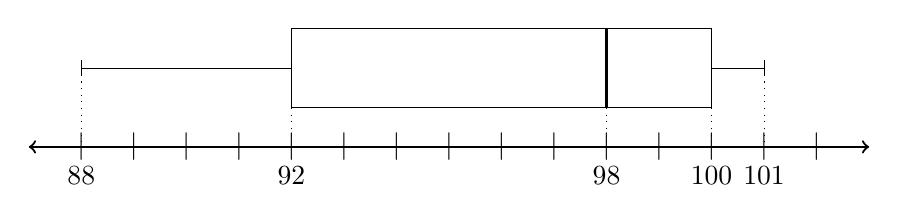
\begin{tikzpicture}[xscale=0.667]
            \def\median{98}
            \def\firstquartile{92}
            \def\thirdquartile{100}
            \def\minimum{88}
            \def\maximum{101}

            \draw (\firstquartile, -0.5 ) rectangle ( \thirdquartile,0.5);
            \draw[thick] ( \median,-0.5) -- ( \median,0.5);
            \draw (    \firstquartile, 0) -- (\minimum,0   );
            \draw ( \minimum, -0.1) -- (       \minimum, 0.1);
            \draw (  \thirdquartile, 0) -- (   \maximum, 0);
            \draw ( \maximum, -0.1) -- (      \maximum, 0.1 );

            \draw[thick,<->] (87,-1) -- (103,-1);

            \foreach \x in {\minimum, \firstquartile, \median, \thirdquartile, \maximum} {
              \draw (\x,-1.6) -- (\x, -1.6) node[anchor=south] {$\x$};
            }

            \foreach \x in {88,89,...,102} {
              \draw (\x,-1.3) -- (\x, -1.3) node[anchor=south] {$|$};
            }
            \draw[dotted] ( \maximum, 0) -- ( \maximum, -1);
            \draw[dotted] ( \thirdquartile, 0) -- ( \thirdquartile, -1);
            \draw[dotted] (\median, 0)  -- ( \median, -1);
            \draw[dotted] (\firstquartile, 0) -- ( \firstquartile, -1);
            \draw[dotted] ( \minimum, 0) -- ( \minimum, -1);
          \end{tikzpicture}
        }
      \end{enumerate}
    \end{enumerate}
}
\end{exercises}


 \begin{solutions}{}{
\begin{enumerate}[itemsep=5pt, label=\textbf{\arabic*}. ] 


\item \\%solution 1
Minimum: $3$ \\
$Q_1$: $17,5$ \\
Mediaan: $27$\\
$Q_3$: $44$\\
Maksimum: $65$\\
\par
\scalebox{0.8}{
    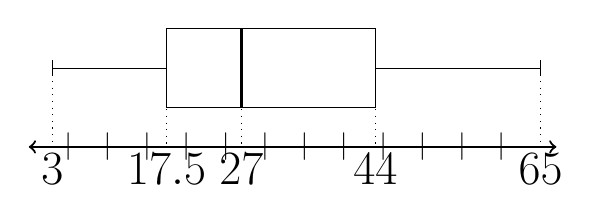
\begin{tikzpicture}[xscale=0.1]
      \def\median{27}
      \def\firstquartile{17.5}
      \def\thirdquartile{44}
      \def\minimum{3}
      \def\maximum{65}

      \draw (\firstquartile, -0.5 ) rectangle ( \thirdquartile,0.5);
      \draw[thick] ( \median,-0.5) -- ( \median,0.5);
      \draw (    \firstquartile, 0) -- (\minimum,0   );
      \draw ( \minimum, -0.1) -- (       \minimum, 0.1);
      \draw (  \thirdquartile, 0) -- (   \maximum, 0);
      \draw ( \maximum, -0.1) -- (      \maximum, 0.1 );

      \draw[thick,<->] (0,-1) -- (67,-1);

      \foreach \x in {\minimum, \firstquartile, \median, \thirdquartile, \maximum} {
        \draw (\x,-1.6) -- (\x, -1.6) node[anchor=south] {\LARGE $\x$};
      }

      \foreach \x in {5,10,...,60} {
        \draw (\x,-1.3) -- (\x, -1.3) node[anchor=south] {$|$};
      }
      \draw[dotted] ( \maximum, 0.09) -- ( \maximum, -1);
      \draw[dotted] ( \thirdquartile, 0.49) -- ( \thirdquartile, -1);
      \draw[dotted] (\median, 0.49)  -- ( \median, -1);
      \draw[dotted] (\firstquartile, 0.49) -- ( \firstquartile, -1);
      \draw[dotted] ( \minimum, 0.09) -- ( \minimum, -1);
    \end{tikzpicture}}

\item %solution 2
Minimum: $1$ \\
$Q_1$: $12$ \\
Mediaan: $28,5$\\
$Q_3$: $46,5$\\
Maksimum: $60$\\
\par
%   sales.
\scalebox{0.8}{
    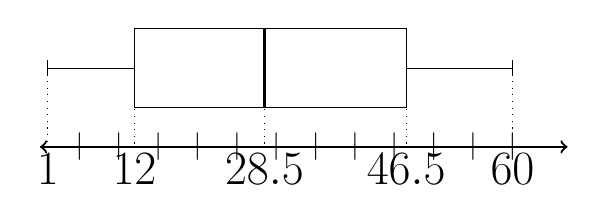
\begin{tikzpicture}[xscale=0.1]
      \def\median{28.5}
      \def\firstquartile{12}
      \def\thirdquartile{46.5}
      \def\minimum{1}
      \def\maximum{60}

      \draw (\firstquartile, -0.5 ) rectangle ( \thirdquartile,0.5);
      \draw[thick] ( \median,-0.5) -- ( \median,0.5);
      \draw (    \firstquartile, 0) -- (\minimum,0   );
      \draw ( \minimum, -0.1) -- (       \minimum, 0.1);
      \draw (  \thirdquartile, 0) -- (   \maximum, 0);
      \draw ( \maximum, -0.1) -- (      \maximum, 0.1 );

      \draw[thick,<->] (0,-1) -- (67,-1);

      \foreach \x in {\minimum, \firstquartile, \median, \thirdquartile, \maximum} {
        \draw (\x,-1.6) -- (\x, -1.6) node[anchor=south] {\LARGE $\x$};
      }

      \foreach \x in {5,10,...,60} {
        \draw (\x,-1.3) -- (\x, -1.3) node[anchor=south] {$|$};
      }
      \draw[dotted] ( \maximum, 0.09) -- ( \maximum, -1);
      \draw[dotted] ( \thirdquartile, 0.49) -- ( \thirdquartile, -1);
      \draw[dotted] (\median, 0.49)  -- ( \median, -1);
      \draw[dotted] (\firstquartile, 0.49) -- ( \firstquartile, -1);
      \draw[dotted] ( \minimum, 0.09) -- ( \minimum, -1);
    \end{tikzpicture}}
\item %solution 3
Minimum: $3$ \\
$Q_1$: $5$ \\
Mediaan: $7$\\
$Q_3$: $13$\\
Maksimum: $16$\\
\item %solution 4
 \begin{enumerate}[itemsep=5pt, label=\textbf{(\alph*)} ]
\item \\
Minimum: $15$ \\
$Q_1$: $22$ \\
Mediaan: $25$\\
$Q_3$: $28$\\
Maksimum: $35$\\

\item \\%
Minimum: $88$ \\
$Q_1$: $92$ \\
Mediaan: $98$\\
$Q_3$: $100$\\
Maksimum: $101$\\   
\end{enumerate}
\end{enumerate}}
\end{solutions}


\begin{eocexercises}{}
  \begin{enumerate}[itemsep=6pt, label=\textbf{\arabic*}.]

  \item 
  Die hoogste $7$ bome in die park het hoogtes (in meters): 
\begin{center} 
 $41$; $60$; $47$; $42$; $44$; $42$; $47$  
\end{center}
Vind die mediaan van hulle hoogtes.

  \item Die studente in Ndeme se klas het die volgende ouderdomme:
    \begin{center} 
$5$; $6$; $7$; $5$; $4$; $6$; $6$; $6$; $7$; $4$ 
    \end{center}
Vind die modale ouderdom.

  \item ’n Ingenieursfirma het twee tipes enjins vir motorfietse ontwerp. Die twee motorfietse word getoets vir die tyd (in sekondes) wat dit hulle neem om te versnel van $0$
    km/h tot $60$ km/h.

    \begin{center}
      \begin{tabular}{|@{\hspace{0.1cm}}c@{\hspace{0.1cm}}|@{\hspace{0.1cm}}c@{\hspace{0.1cm}}|@{\hspace{0.1cm}}c@{\hspace{0.1cm}}|@{\hspace{0.1cm}}c@{\hspace{0.1cm}}|@{\hspace{0.1cm}}c@{\hspace{0.1cm}}|@{\hspace{0.1cm}}c@{\hspace{0.1cm}}|@{\hspace{0.1cm}}c@{\hspace{0.1cm}}|@{\hspace{0.1cm}}c@{\hspace{0.1cm}}|@{\hspace{0.1cm}}c@{\hspace{0.1cm}}|@{\hspace{0.1cm}}c@{\hspace{0.1cm}}|@{\hspace{0.1cm}}c@{\hspace{0.1cm}}|} \hline
     
        & \textbf{Toets 1} & \textbf{Toets 2} & \textbf{Toets 3} & \textbf{Toets 4} & \textbf{Toets 5} & \textbf{Toets 6} & \textbf{Toets 7} &\textbf{Toets 8} & \textbf{Toets 9} & \textbf{Toets 10} \\\hline
        \textbf{Fiets 1} & $1,55$ & $1,00$ & $0,92$ & $0,80$ & $1,49$ & $0,71$ & $1,06$ & $0,68$ & $0,87$ & $1,09$ \\\hline
        \textbf{Fiets 2} & $0,9$ & $1,0$ & $1,1$ & $1,0$ & $1,0$ & $0,9$ & $0,9$ & $1,0$ & $0,9$ & $1,1$ \\\hline

      \end{tabular}
    \end{center}
\vspace {8pt}\\
\begin{enumerate}[noitemsep, label=\textbf{(\alph*)} ]
    \item Watter maatstaf van sentrale neiging behoort gebruik te word vir hierdie data?
    \item Bereken die maatstaf van sentrale neiging wat jy gekies het in (a), vir elke motorfiets.
    \item Watter motorfiets sou jy kies, gebaseer op hierdie inligting? Neem kennis van die akkuraatheid van die getalle in elke stel toetse. 
      
    \end{enumerate}

  \item In ’n verkeersopname, word ’n willekeurige steekproef van $50$ motoriste gevra oor die afstand wat hulle elke dag werk toe ry. Die informasie word getoon in die tabel hieronder: \\
    \begin{center}
      \begin{tabular}{|c|c|} \hline
     
        \textbf{Afstand (km)} & \textbf{Telling} \\ \hline

        $0 < d \leq 5$ & $4$ \\ \hline
        $5 < d \leq 10$ & $5$ \\\hline
        $10 < d \leq 15$ & $9$ \\\hline
        $15 < d \leq 20$ & $10$ \\\hline
        $20 < d \leq 25$ & $7$ \\\hline
        $25 < d \leq 30$ & $8$ \\\hline
        $30 < d \leq 35$ & $3$ \\\hline
        $35 < d \leq 40$ & $2$ \\\hline
        $40 < d \leq 45$ & $2$ \\\hline

      \end{tabular}
    \end{center}
\vspace {8pt}\\
     \begin{enumerate}[noitemsep, label=\textbf{(\alph*)} ]
    \item Vind die benaderde gemiddelde van die data.
    \item Watter persentasie van die steekproef ry 
      \begin{enumerate}[noitemsep, label=\textbf{\roman*}. ]
      \item minder as $15$ km?
      \item meer as $30$ km?
      \item tussen $16$ km en $30$ km daagliks?
      \end{enumerate}
\item Teken 'n histogram om die data voor te stel.
    \end{enumerate}

  \item ’n Maatskappy wil die opleidingsprogram in sy fabriek evalueer. Hulle gee dieselfde taakopdrag aan opgeleide en onopgeleide werknemers en meet die tyd in sekondes wat  dit die werkers neem om die taak te voltooi. 
\\
    \begin{center}
      \begin{tabular}{|l|c|c|c|c|c|} \hline

        \textbf{Opgeleide} & 121 & 137 & 131 & 135 & 130 \\ \hline
                         & 128 & 130 & 126 & 132 & 127 \\\hline
                         & 129 & 120 & 118 & 125 & 134 \\\hline

        \textbf{Onopgeleide} & 135 & 142 & 126 & 148 & 145 \\\hline
                           & 156 & 152 & 153 & 149 & 145 \\\hline
                           & 144 & 134 & 139 & 140 & 142 \\\hline

      \end{tabular}
    \end{center}
\vspace {8pt}\\
    \begin{enumerate}[noitemsep, label=\textbf{(\alph*)} ]
    \item Vind die mediane en kwartiele vir beide stelle data.
    \item Vind die interkwartielwydtes vir beide stelle data.
    \item Lewer kommentaar op die resultate.
\item Teken 'n mond-en-snor diagram wat die vyf-getal-opsomming illustreer, vir elke datastel.
    \end{enumerate}

  \item ’n Klein firma het $9$ mense in diens. Die jaarlikse salarisse van die werknemers is:\\
    \begin{center}
      \begin{tabular}{|r|r|r|} \hline
        R~$600~000$ & R~$250~000$ & R~$200~000$ \\\hline
        R~$120~000$ & R~$100~000$ & R~$100~000$ \\\hline
        R~$100~000$ &  R~$90~000$ &  R~$80~000$ \\\hline
      \end{tabular}
    \end{center}
\vspace {8pt}\\
    \begin{enumerate}[noitemsep, label=\textbf{(\alph*)} ]
    \item Vind die gemiddelde van hierdie salarisse
    \item Vind die modus
    \item Vind die mediaan
    \item Watter een van die drie getalle sou jy gebruik om te onderhandel oor salarisverhogings as jy ’n vakbondbeampte is? Waarom?
    \end{enumerate}

  \end{enumerate}

\end{eocexercises}


 \begin{eocsolutions}{}{
\begin{enumerate}[itemsep=5pt, label=\textbf{\arabic*}. ] 


\item %solution 1
Mediaan $=\dfrac{41+60+47+42+44+42+47}{7} \\
~~~~~~~~=44$
\item %solution 2
Modus $=6$
\item %solution 3

\begin{enumerate}[noitemsep, label=\textbf{(\alph*)} ]
    \item Gemiddelde en modus. Die gemiddelde sal ons die gemiddelde versnelling tyd gee, tensy die modus ons die tyd wat die meeste verkry is sal gee.%What measure of central tendency should be used for this
%       information?
    \item Vir fiets $1$ die gemiddelde is $1,02$ s en daar is nie 'n modus nie want daar is geen waarde wat meer as een keer plaasvind.\\
	  Vir fiets $2$ die gemiddelde is  $1,0$ s en daar is twee modi $1,0$ en $0,9$.
    \item Dit sal mooilik wees om te kies. Alhoewel fiets $1$ blyk om beter te doen as fiets $2$ van die gemiddelde af, die data vir fiets $2$ is minder akkuraat as dié vir fiest $1$ (dit het net een desimale plek). As ons die gemiddelde vir fiets $1$ bereken om deur net $1$ desimale plek te gebruik, sal ons $0,9$ s kry. Dit sal fiets $2$ beter maak. Verder, fiets $2$ lewer meer konsekwent getalle. Dus sal fiest $2$ waarskynlik 'n beter keuse wees, maar meer inligting of meer akkurate inligting verkry moet word.

    \end{enumerate}

\item %solution 4
 \begin{enumerate}[noitemsep, label=\textbf{(\alph*)} ]
    \item Gemiddelde $=\dfrac{4(3)+5(8)+9(13)+10(18)+7(23)+8(28)+3(33)+2(38)+2(43)}{50}\\
~~~~~~=19,9$
    \item %What percentage of samples had a speed of
      \begin{enumerate}[noitemsep, label=\textbf{\roman*}. ]
      \item Daar was $18$ bestuurders wat minder as $15$ km gery het.\\
	    Dus $\frac{18}{50}\times 100 = 38\%$%less than $15$ km?
      \item Daar was $7$ bestuurders wat minder as $30$ km gery het.\\
	    Dus $\frac{7}{50}\times 100 = 14\%$%more than $30$ km?
      \item $100-(36-14) = 50\%$%between $16$ km and $30$ km daily?
      \end{enumerate}
\item %Draw a histogram to represent the data
\scalebox{0.8} % Change this value to rescale the drawing.
{
\begin{pspicture}(0,-3.62375)(11.17442,3.58375)
\definecolor{color6331b}{rgb}{0.7725490196078432,0.7725490196078432,0.7725490196078432}
\psframe[linewidth=0.02,dimen=outer,fillstyle=solid,fillcolor=color6331b](2.208587,-0.41625)(1.1885868,-2.4128125)
\rput(1.1744202,-2.41625){\psaxes[linewidth=0.028222222,arrowsize=0.05291667cm 2.0,arrowlength=1.4,arrowinset=0.4,tickstyle=bottom,ticksize=0.10583333cm,dx=1.0cm,dy=0.5cm,Dx=5]{<->}(0,0)(-1,-1)(10,6)}
\psframe[linewidth=0.02,dimen=outer,fillstyle=solid,fillcolor=color6331b](3.188587,0.10375)(2.168587,-2.4128125)
\psframe[linewidth=0.02,dimen=outer,fillstyle=solid,fillcolor=color6331b](4.2085867,2.10375)(3.168587,-2.4128125)
\psframe[linewidth=0.02,dimen=outer,fillstyle=solid,fillcolor=color6331b](5.2085867,2.60375)(4.1685867,-2.4128125)
\psframe[linewidth=0.02,dimen=outer,fillstyle=solid,fillcolor=color6331b](6.1885867,1.12375)(5.1685867,-2.4128125)
\psframe[linewidth=0.02,dimen=outer,fillstyle=solid,fillcolor=color6331b](7.1885867,1.58375)(6.1685867,-2.4128125)
% \usefont{T1}{ptm}{m}{n}
\rput(6.062962,-3.42625){\LARGE Afstand (km)}
% \usefont{T1}{ptm}{m}{n}
\rput{89.854546}(1.2403736,0.9631185){\rput(0.11709099,1.0822288){\LARGE Telling}}
\psframe[linewidth=0.02,dimen=outer,fillstyle=solid,fillcolor=color6331b](8.188587,-0.89625)(7.1685867,-2.4128125)
\psframe[linewidth=0.02,dimen=outer,fillstyle=solid,fillcolor=color6331b](9.188587,-1.39625)(8.168587,-2.4128125)
\psframe[linewidth=0.02,dimen=outer,fillstyle=solid,fillcolor=color6331b](10.188587,-1.39625)(9.168587,-2.4128125)
\end{pspicture} 
}
\end{enumerate}}
\item %solution 5
\begin{enumerate}[noitemsep, label=\textbf{(\alph*)} ]
\item
Eerstens, orde die datastelle vir albei opgeleide en onopgeleide personeel.\\
Opgeleide: $118, 120, 121, 125, 126, 127, 128, 129, 130, 130, 131, 132, 134, 135, 137$ \\
Onopgeleide: $126, 134, 135, 139, 140, 142, 142, 144, 145, 145, 148, 149, 152, 153, 156$ \\
Daar is $15$ waardes in elke datastel. \\
Posisie van die mediaan is $\frac{15+1}{2}=8$. \\
Vir die opgeleide personeel is dit $129$ en vir die onopgeleide personeel is dit $144$.\\
Posisies van die kwartiele is $\frac{15}{4}=3,75$.\\
Vir die opgeleide personeel: $Q_1=125$ en $Q_3=132$.\\
Vir die onopgeleide personeel: $Q_1=139$ en $Q_3=149$.\\
\item
Interkwartielwydte vir die opgeleide personeel: $Q_3-Q_1=7$.\\
Interkwartielwydte vir die onopgeleide personeel: $Q_3-Q_1=10$.\\
\item
Die mediaan van die onopgeleide personeel is hoër as dié  van die onopgeleide personeel. Verder, die onopgeleide personeel get 'n groter interkwartielwydte as die opgeleide personeel. Daar is 'n paar bewyse dat die opleidingsprogram mag werk.
\item %Draw two box-and-whisker diagrams to illustrate the five number summary
Opgeleide personeel:\\
\scalebox{0.5}{
    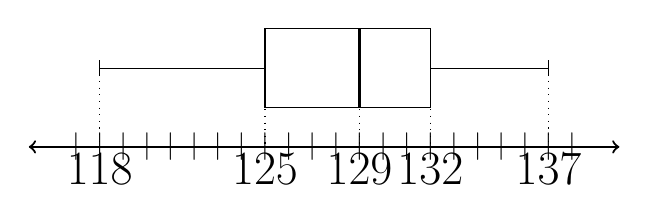
\begin{tikzpicture}[xscale=0.3]
      \def\median{129}
      \def\firstquartile{125}
      \def\thirdquartile{132}
      \def\minimum{118}
      \def\maximum{137}

      \draw (\firstquartile, -0.5 ) rectangle ( \thirdquartile,0.5);
      \draw[thick] ( \median,-0.5) -- ( \median,0.5);
      \draw (    \firstquartile, 0) -- (\minimum,0   );
      \draw ( \minimum, -0.1) -- (       \minimum, 0.1);
      \draw (  \thirdquartile, 0) -- (   \maximum, 0);
      \draw ( \maximum, -0.1) -- (      \maximum, 0.1 );

      \draw[thick,<->] (115,-1) -- (140,-1);

      \foreach \x in {\minimum, \firstquartile, \median, \thirdquartile, \maximum} {
        \draw (\x,-1.6) -- (\x, -1.6) node[anchor=south] {\LARGE$\x$};
      }

      \foreach \x in {117,118,...,138} {
        \draw (\x,-1.3) -- (\x, -1.3) node[anchor=south] {$|$};
      }
      \draw[dotted] ( \maximum, 0.09) -- ( \maximum, -1);
      \draw[dotted] ( \thirdquartile, 0.49) -- ( \thirdquartile, -1);
      \draw[dotted] (\median, 0.49)  -- ( \median, -1);
      \draw[dotted] (\firstquartile, 0.49) -- ( \firstquartile, -1);
      \draw[dotted] ( \minimum, 0.09) -- ( \minimum, -1);
    \end{tikzpicture}}
  
\\
Onopgeleide werknemers:\\
\scalebox{0.5}{
    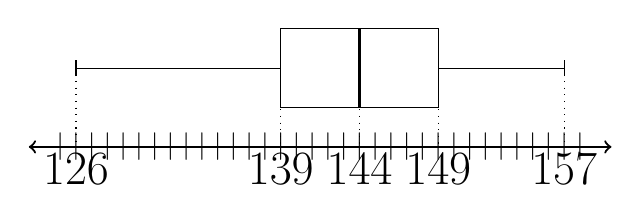
\begin{tikzpicture}[xscale=0.2]
      \def\median{144}
      \def\firstquartile{139}
      \def\thirdquartile{149}
      \def\minimum{126}
      \def\maximum{157}

      \draw (\firstquartile, -0.5 ) rectangle ( \thirdquartile,0.5);
      \draw[thick] ( \median,-0.5) -- ( \median,0.5);
      \draw (    \firstquartile, 0) -- (\minimum,0   );
      \draw ( \minimum, -0.1) -- (       \minimum, 0.1);
      \draw (  \thirdquartile, 0) -- (   \maximum, 0);
      \draw ( \maximum, -0.1) -- (      \maximum, 0.1 );

      \draw[thick,<->] (123,-1) -- (160,-1);

      \foreach \x in {\minimum, \firstquartile, \median, \thirdquartile, \maximum} {
        \draw (\x,-1.6) -- (\x, -1.6) node[anchor=south] {\LARGE$\x$};
      }

      \foreach \x in {125,126,...,158} {
        \draw (\x,-1.3) -- (\x, -1.3) node[anchor=south] {$|$};
      }
      \draw[dotted] ( \maximum, 0.09) -- ( \maximum, -1);
      \draw[dotted] ( \thirdquartile, 0.49) -- ( \thirdquartile, -1);
      \draw[dotted] (\median, 0.49)  -- ( \median, -1);
      \draw[dotted] (\firstquartile, 0.49) -- ( \firstquartile, -1);
      \draw[dotted] ( \minimum, 0.09) -- ( \minimum, -1);
    \end{tikzpicture}}
\end{enumerate}
\item %solution 6
\begin{enumerate}[noitemsep, label=\textbf{(\alph*)} ]
\item
Gemiddelde $=\frac{1~640~000}{9}=182~222,22$
\item
Modus is R $100~000$.
\item
 Eerstens, orde die datastelle. Om dit maklier om met die getalle te werk, deel ons elkeen deur $100~000$.\\
Die geordende stel is $80, 90, 100, 100, 100, 120, 200, 250, 600$.  \\
Die mediaan is by posisie $5$ en R $100~000$ is.
\item
Óf die modus of die mediaan. \\
Die gemiddelde is deur die een salaris van R $600~000$ geskeedf(verskuif). Die modus gee ons 'n beter raming van wat die personeel eintlik verdien. 
Die mediaan gee ons ook 'n redelike akkurate voorstelling van wat die personeel verdien.


\end{enumerate}
}
\end{eocsolutions}


